%%%%%%%%%%%%%%%%%%%%%%%%%%%%%%%%%%%%%%%%%%%%%%%%%%%%%%%%%%%%%%%%%%%%%%%%%%%%%%%
\documentclass[hyperref={pdfpagelabels=false},compress,table]{beamer} % 在Mac下无法编译
% \documentclass[compress,table]{beamer} % 在Mac下使用
% package for font
\usepackage{fontspec}
\defaultfontfeatures{Mapping=tex-text}  %%如果没有它,会有一些 tex 特殊字符无法正常使用,比如连字符。
\usepackage{xunicode,xltxtra}
\usepackage[BoldFont,SlantFont,CJKnumber,CJKchecksingle]{xeCJK}  % \CJKnumber{12345}: 一万二千三百四十五
\usepackage{CJKfntef}  %%实现对汉字加点、下划线等。
\usepackage{pifont}  % \ding{}
% package for math
\usepackage{amsfonts}

% package for graphics
\usepackage[americaninductors,europeanresistors]{circuitikz}
\usepackage{tikz}
\usetikzlibrary{plotmarks}  % placements=positioning
\usepackage{graphicx}  % \includegraphics[]{}
\usepackage{subfigure}  %%图形或表格并排排列
% package for table
\usepackage{colortbl,dcolumn}  %% 彩色表格
\usepackage{multirow}
\usepackage{multicol}
\usepackage{booktabs}
% package for code
\usepackage{fancyvrb}
\usepackage{listings}

% \usepackage{animate}
% \usepackage{movie15}

%%%%%
% setting for beamer
\usetheme{default} % Madrid(常用), Copenhagen, AnnArbor, boxes(白色), Frankfurt,Berkeley
\useoutertheme[subsection=true]{miniframes} % 使用Berkeley时注释本行
\usecolortheme{sidebartab}
\usefonttheme{serif}  %%英文使用衬线字体
% \setbeamertemplate{background canvas}[vertical
% shading][bottom=white,top=structure.fg!7] %%背景色,上25%的蓝,过渡到下白。
\setbeamertemplate{theorems}[numbered]
\setbeamertemplate{navigation symbols}{}  %% 去掉页面下方默认的导航条
\setbeamercovered{transparent}  %设置 beamer 覆盖效果

% 设置标题title背景色
% \setbeamercolor{title}{fg=black, bg=lightgray!60!white}
\setbeamercolor{title}{fg=white, bg=black!70!white}

% 设置每页小LOGO
\pgfdeclareimage[width=1cm]{ouc}{figures/static/ouc.pdf}
\logo{\pgfuseimage{ouc}{\vspace{-20pt}}}

% setting for font
%%\setCJKmainfont{Adobe Kaiti Std}
\setCJKmainfont{SimSun} 
%% \setCJKmainfont{FangSong_GB2312} 
%% \setmainfont{Apple Garamond}  %%苹果字体没有SmallCaps
\setCJKmainfont{SimSun} 
%FUNNY%\setCJKmainfont{DFPShaoNvW5-GB}  %%华康少女文字W5(P)
%FUNNY%\setCJKmainfont{FZJingLeiS-R-GB}  %%方正静蕾体
%FUNNY%\setmainfont{Purisa}
%\setsansfont[Mapping=tex-text]{Adobe Song Std}
     %如果装了Adobe Acrobat,可在font.conf中配置Adobe字体的路径以使用其中文字体。
     %也可直接使用系统中的中文字体如SimSun、SimHei、微软雅黑等。
     %原来beamer用的字体是sans family;注意Mapping的大小写,不能写错。
     %设置字体时也可以直接用字体名,以下三种方式等同:
     %\setromanfont[BoldFont={黑体}]{宋体}
     %\setromanfont[BoldFont={SimHei}]{SimSun}
     %\setromanfont[BoldFont={"[simhei.ttf]"}]{"[simsun.ttc]"}
% setting for graphics
\graphicspath{{figures/}}  %%图片路径
\renewcommand\figurename{图}

% setting for pdf
\hypersetup{% pdfpagemode=FullScreen,%
            pdfauthor={Xiaodong Wang},%
            pdftitle={Title},%
            CJKbookmarks=true,%
            bookmarksnumbered=true,%
            bookmarksopen=false,%
            plainpages=false,%
            colorlinks=true,%
            citecolor=green,%
            filecolor=magenta,%
            linkcolor=blue,%red(default)
            urlcolor=cyan}

% setting for fontspec
\XeTeXlinebreaklocale "zh"  %%表示用中文的断行
\XeTeXlinebreakskip = 0pt plus 1pt minus 0.1pt  %%多一点调整的空间
%%%%%

% font setting by xeCJK
\setCJKfamilyfont{NSimSun}{NSimSun}
\newcommand{\song}{\CJKfamily{NSimSun}}
%%%\setCJKfamilyfont{AdobeSongStd}{Adobe Song Std}
%%%\newcommand{\AdobeSong}{\CJKfamily{AdobeSongStd}}
\setCJKfamilyfont{FangSong}{FangSong_GB2312}
\newcommand{\fang}{\CJKfamily{FangSong}}
%%%\setCJKfamilyfont{AdobeFangsongStd}{Adobe Fangsong Std}
%%%\newcommand{\AdobeFang}{\CJKfamily{AdobeFangsongStd}}
\setCJKfamilyfont{SimHei}{SimHei}
\newcommand{\hei}{\CJKfamily{SimHei}}
%%%\setCJKfamilyfont{AdobeHeitiStd}{Adobe Heiti Std}
%%%\newcommand{\AdobeHei}{\CJKfamily{AdobeHeitiStd}}
\setCJKfamilyfont{KaiTi}{KaiTi}
\newcommand{\kai}{\CJKfamily{KaiTi}}
%%%\setCJKfamilyfont{AdobeKaitiStd}{Adobe Kaiti Std}
\newcommand{\AdobeKai}{\CJKfamily{AdobeKaitiStd}}
\setCJKfamilyfont{LiSu}{LiSu}
\newcommand{\li}{\CJKfamily{LiSu}}
\setCJKfamilyfont{YouYuan}{YouYuan}
\newcommand{\you}{\CJKfamily{YouYuan}}
\setCJKfamilyfont{FZJingLei}{FZJingLeiS-R-GB}
\newcommand{\jinglei}{\CJKfamily{FZJingLei}}
\setCJKfamilyfont{MSYH}{Microsoft YaHei}
\newcommand{\msyh}{\CJKfamily{MSYH}}

% 自定义颜色
\def\Red{\color{red}}
\def\Green{\color{green}}
\def\Blue{\color{blue}}
\def\Mage{\color{magenta}}
\def\Cyan{\color{cyan}}
\def\Brown{\color{brown}}
\def\White{\color{white}}
\def\Black{\color{black}}

\lstnewenvironment{xmlCode}[1][]{% for Java
  \lstset{
    basicstyle=\tiny\ttfamily,%
    columns=flexible,%
    framexleftmargin=.7mm, %
    % frame=shadowbox,%
    % rulesepcolor=\color{cyan},%
     frame=single,%
    backgroundcolor=\color{white},%
    xleftmargin=4\fboxsep,%
    xrightmargin=4\fboxsep,%
    numbers=left,numberstyle=\tiny,%
    numberblanklines=false,numbersep=7pt,%
    language=xml, %
    }\lstset{#1}}{}

\lstnewenvironment{javaCode}[1][]{% for Java
  \lstset{
    basicstyle=\tiny\ttfamily,%
    columns=flexible,%
    framexleftmargin=.7mm, %
    frame=shadowbox,%
    rulesepcolor=\color{cyan},%
    % frame=single,%
    backgroundcolor=\color{white},%
    xleftmargin=4\fboxsep,%
    xrightmargin=4\fboxsep,%
    numbers=left,numberstyle=\tiny,%
    numberblanklines=false,numbersep=7pt,%
    language=Java, %
    }\lstset{#1}}{}

\lstnewenvironment{shCode}[1][]{% for Java
  \lstset{
    basicstyle=\scriptsize\ttfamily,%
    columns=flexible,%
    framexleftmargin=.7mm, %
    frame=shadowbox,%
    rulesepcolor=\color{brown},%
    % frame=single,%
    backgroundcolor=\color{white},%
    xleftmargin=4\fboxsep,%
    xrightmargin=4\fboxsep,%
    numbers=left,numberstyle=\tiny,%
    numberblanklines=false,numbersep=7pt,%
    language=sh, %
    }\lstset{#1}}{}

\newcommand\ask[1]{\vskip 4bp \tikz \node[rectangle,rounded corners,minimum size=6mm,
  fill=white,]{\Cyan \includegraphics[height=1.5cm]{question} \Large \msyh #1};}

\newcommand\wxd[1]{\vskip 4bp \tikz \node[rectangle,minimum size=6mm,
  fill=blue!60!white,]{\White \ding{118} \msyh #1};}

\newcommand\xyy[1]{\vskip 2bp \tikz \node[rectangle,minimum size=3mm,
  fill=black!80!white,]{\White \msyh\scriptsize #1};}

\newcommand\cxf[1]{\vskip 4bp \tikz \node[rectangle,rounded corners,minimum size=6mm,
  fill=orange!60!white,]{\White \ding{42} \msyh #1};}

\newcommand\samp[1]{\vskip 2bp \tikz \node[rectangle,minimum size=3mm,
  fill=white!100!white,]{\Mage\msyh \small CODE \ding{231} \Black #1};\vskip -8bp}

\newcommand\zhyfly[1]{\tikz \node[rectangle,rounded corners,minimum size=6mm,ball color=red!25!blue,text=white,]{#1};}

\setbeamerfont{frametitle}{series=\msyh} % 修改Beamer标题字体

\makeatletter
\newcommand{\Extend}[5]{\ext@arrow 0099{\arrowfill@#1#2#3}{#4}{#5}}
\makeatother


%%%%%%%%%%%%%%%%%%%%%%%%%%%%%%%%%%%%%%%%%%%%%%%%%%%%%%%%%%%%%%%%%%%%%%%%%%%%%%%
\title[JAVA]{\hei {\huge Java 应用与开发}\\  
 Java内存模型与分配机制}
\author[王晓东]{王晓东\\
  \href{mailto:wangxiaodong@ouc.edu.cn}{\footnotesize wangxiaodong@ouc.edu.cn}}
\institute[中国海洋大学]{\small 中国海洋大学}
\date{\today}
\titlegraphic{\vspace{-6em}
\includegraphics[height=6cm]{static/ouc.pdf}\vspace{-6em}}
%%%%%%%%%%%%%%%%%%%%%%%%%%%%%%%%%%%%%%%%%%%%%%%%%%%%%%%%%%%%%%%%%%%%%%%%%%%%%%%
\begin{document}
%% Delete this, if you do not want the table of contents to pop up at
%% the beginning of each subsection:
\AtBeginSection[]{                              % 在每个Section前都会加入的Frame
  \frame<handout:0>{
    \frametitle{\textbf{\hei 接下来…}}
    \tableofcontents[currentsection]
  }
}  %

\AtBeginSubsection[]                            % 在每个子段落之前
{
  \frame<handout:0>                             % handout:0 表示只在手稿中出现
  {
    \frametitle{\textit{\hei 接下来…}}\small
    \tableofcontents[current,currentsubsection] % 显示在目录中加亮的当前章节
  }
}
\frame{\titlepage}
%%%%%%%%%%%%%%%%%%%%%%%%%%%%%%%%%%%%%%%%%%%%%%%%

\begin{frame}
  \frametitle{学习目标}
  
  \begin{enumerate}
  \item 理解JVM内存模型,掌握JVM内存构成
  \item 理解Java程序的运行过程,学会通过调试模式观察内存的变化
  \item 了解Java内存管理,认识垃圾回收
  \item 建立编程时高效利用内存、避免内存溢出的理念
  \end{enumerate}  
\end{frame}


\section*{大纲}
\frame{\frametitle{大纲} \tableofcontents }

\section{Java内存模型}

\begin{frame}[fragile] % [fragile]参数使得能够插入代码
  \frametitle{Java虚拟机(Java Virtual Machine, JVM)}
  
  \begin{itemize}\small
  \item Java程序运行在JVM上,JVM是程序与操作系统之间的桥梁。
  \item JVM实现了Java的平台无关性。
  \item JVM是内存分配的前提。
  \end{itemize}

  \begin{figure}
    \centering
    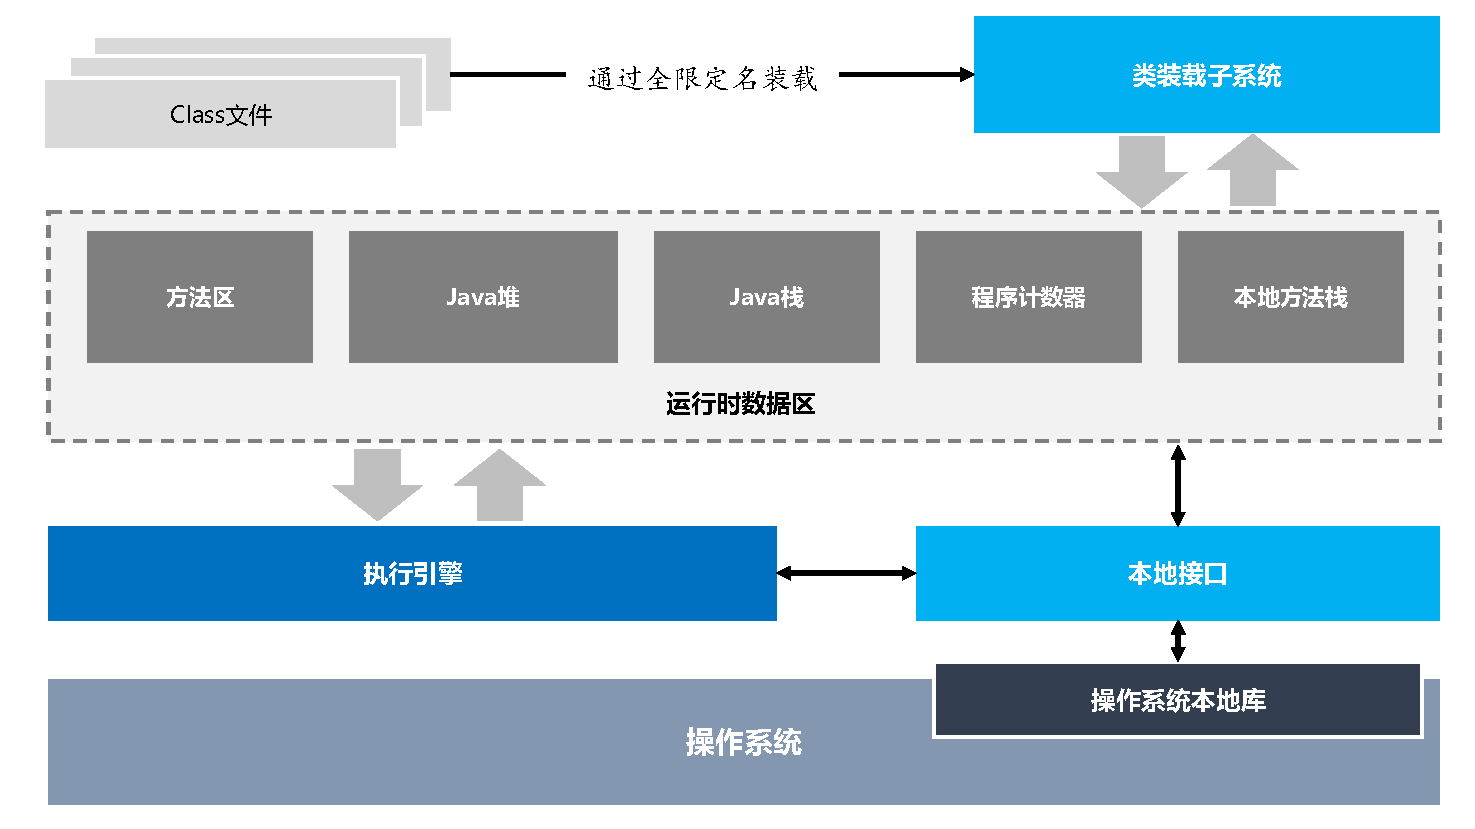
\includegraphics[width=0.9\textwidth]{fig-jvm-arch.pdf}
  \end{figure}
\end{frame}

\begin{frame}[fragile] % [fragile]参数使得能够插入代码
  \frametitle{JVM内存模型}

  \pptlink{./ppt/fig-java-memory-arch.pptx}{JVM内存模型}
  
  \begin{figure}
    \centering
    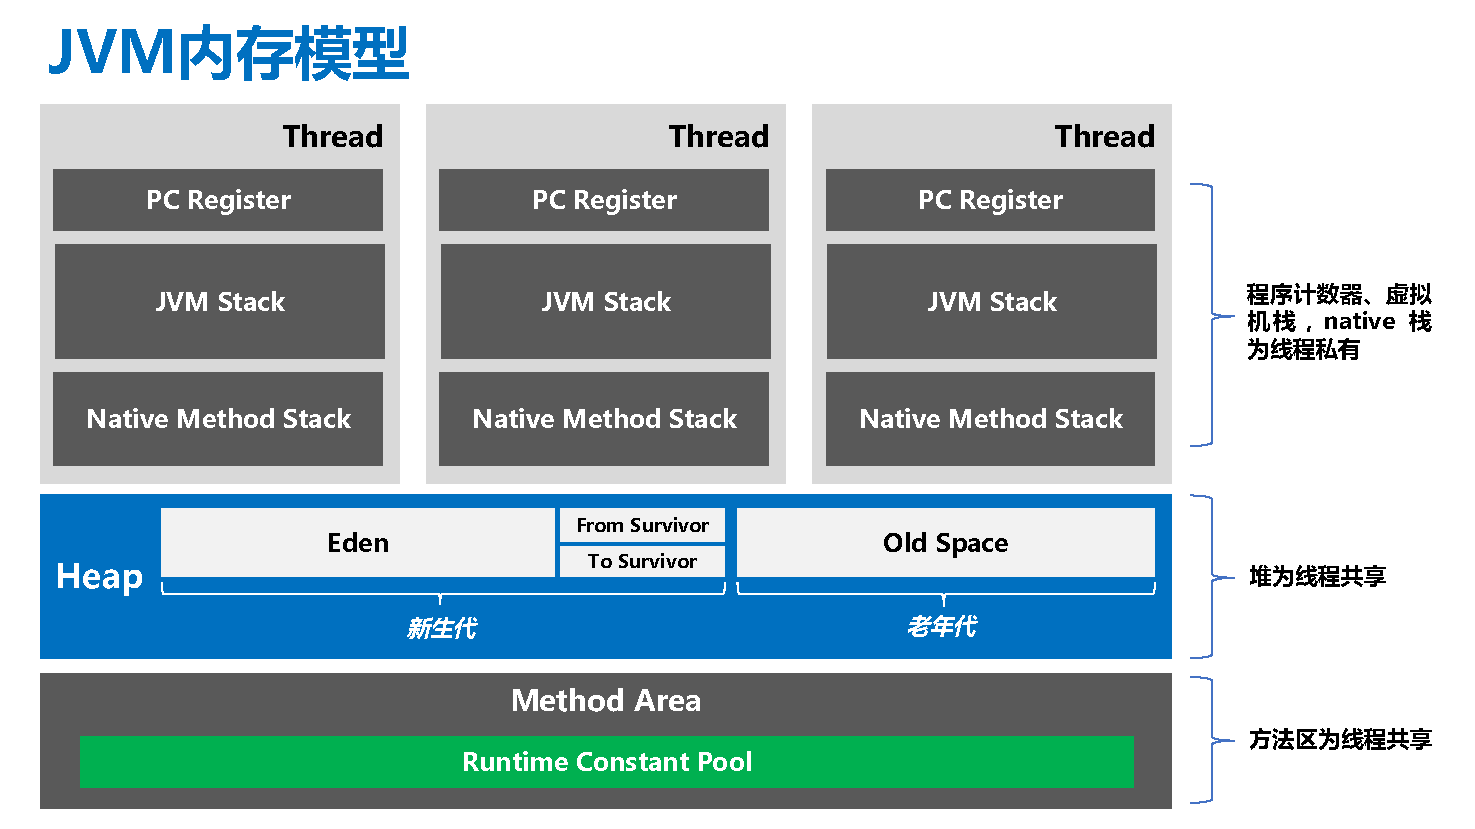
\includegraphics[width=\textwidth]{fig-java-memory-arch.pdf}
  \end{figure}
\end{frame}

%%%\begin{frame}[fragile] % [fragile]参数使得能够插入代码
%%%\frametitle{Java程序运行过程会涉及的内存区域}
%%%\begin{itemize}
%%%\item Permanent space里存放加载的Class类级对象如class本身、method、field等。
%%%\item Heap space主要存放对象和数组。\\
%%%  \only<2>{\kai Heap space由Old Generation和New Generation组成,Old
%%%    Generation存放生命周期长久的实例对象,而新的对象实例一般放在New
%%%    Generation。New Generation还可以再分为Eden区和Survivor区,新的对象
%%%    实例总是首先放在Eden区,Survivor区作为Eden区和Old区的缓冲,可以
%%%    向Old区转移活动的对象实例。}
%%%\end{itemize}
%%%\end{frame}
%%%
%%%\begin{frame}[fragile] % [fragile]参数使得能够插入代码
%%%\frametitle{JVM堆内存空间申请流图}
%%%
%%%\begin{figure}
%%%\centering
%%%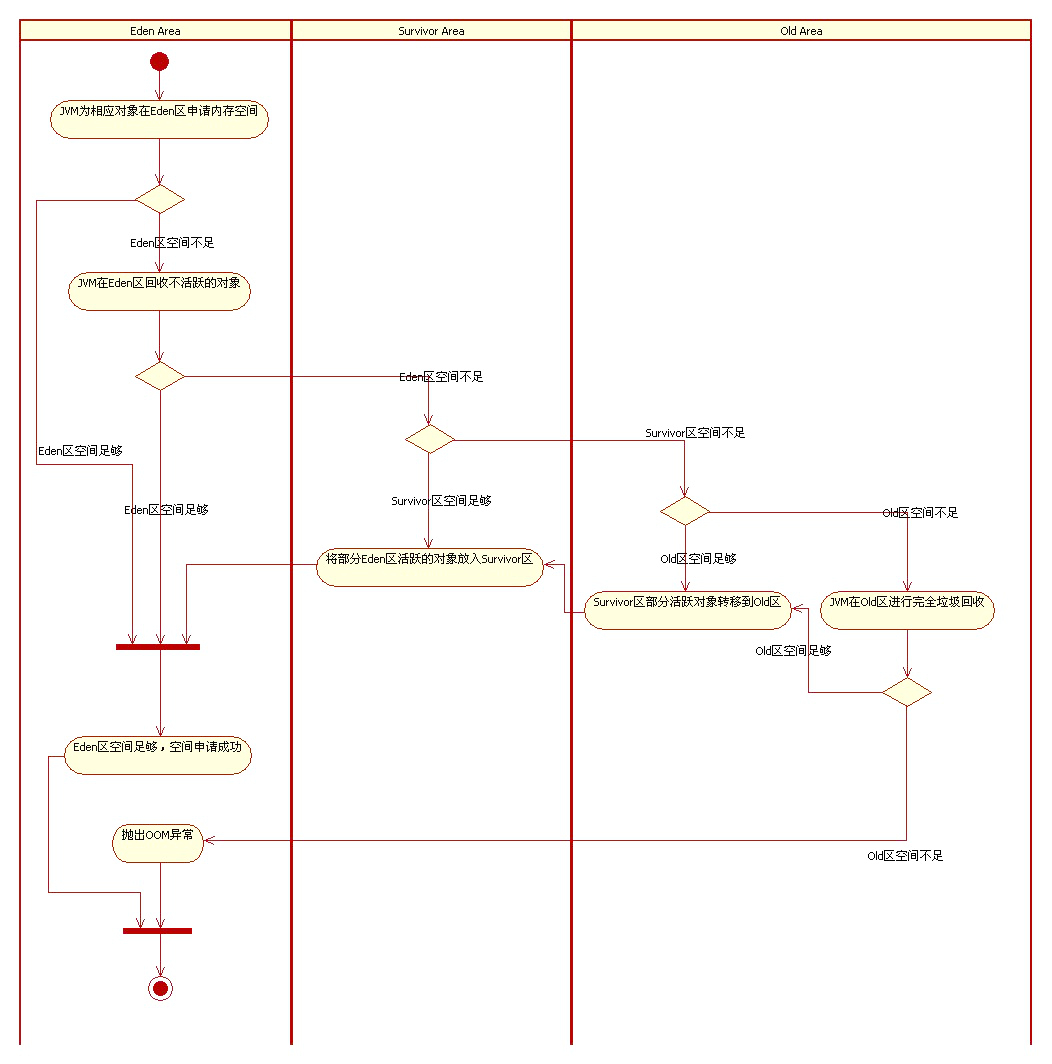
\includegraphics[width=0.6\textwidth]{jmmflow.jpg}
%%%\end{figure}
%%%\end{frame}

\begin{frame}[fragile] % [fragile]参数使得能够插入代码
\frametitle{Java程序运行过程会涉及的内存区域}
\begin{description}[<+-| structure@+>]\kai\small
\item[程序计数器] 当前线程执行的字节码的行号指示器。
\item[栈] 保存局部变量的值,包括:用来保存基本数据类型的值;保存类的实例,即堆区对象的引
  用(指针),也可以用来保存加载方法时的帧。(Stack)
\item[堆] 用来存放动态产生的数据,如new出来的对象和数组。\footnote{注意
    创建出来的对象只包含属于各自的成员变量,并不包括成员方法。因为同一
    个类的对象拥有各自的成员变量,存储在各自的堆内存中,但是他们共享该
    类的方法,并不是每创建一个对象就把成员方法复制一次。}。(Heap)
\item[常量池] JVM为每个已加载的类型维护一个常量池,常量池就是这个类型用到的常量的一个有序
  集合。包括直接常量(基本类型、String)和对其他类型、方法、字段的符号引用。池中的数据和
  数组一样通过索引访问,常量池在Java程序的动态链接中起了核心作用。(Perm)
\item[代码段] 存放从硬盘上读取的源程序代码。(Perm)
\item[数据段] 存放static定义的静态成员。{\Red (Perm)} 
\end{description}
\end{frame}


\section{Java程序内存运行分析}

\begin{frame}[fragile] % [fragile]参数使得能够插入代码
\frametitle{预备知识}

\begin{enumerate}[<+-| structure@+>]
\item 一个Java文件,只要有main入口方法,即可认为这是一个Java程序,可以
  单独编译运行。
\item 无论是普通类型的变量还是引用类型的变量(俗称实例),都可以作为局
  部变量,他们都可以出现在栈中。
\item 普通类型的变量在栈中直接保存它所对应的值,而引用类型的变量保存的
  是一个指向堆区的指针。通过这个指针,就可以找到这个实例在堆区对应的对
  象。因此,{\hei\Red 普通类型变量只在栈区占用一块内存,而引用类型变量
    要在栈区和堆区各占一块内存}。
\end{enumerate}
\end{frame}

\begin{frame}[fragile] % [fragile]参数使得能够插入代码
\frametitle{所用讲解程序示例}
\samp{Test.java}
\begin{javaCode}
public class Test {
  public static void main(String[] args) {
    Test test = new Test();
    int data = 9;
    BirthDate d1 = new BirthDate(22, 12, 1982);
    BirthDate d2 = new BirthDate(10, 10, 1958);
    test.m1(data);
    test.m2(d1);
    test.m3(d2);
  }

  public void m1(int i) {
    i = 1234;
  }
  public void m2(BirthDate b) {
    b = new BirthDate(15, 6, 2010);
  }
  public void m3(BirthDate b) {
    b.setDay(18);
  }
}
\end{javaCode}
\end{frame}

\begin{frame}[fragile] % [fragile]参数使得能够插入代码
\frametitle{程序调用过程(一)}

\begin{columns}
\column{0.4\textwidth} 
\begin{figure}
\centering
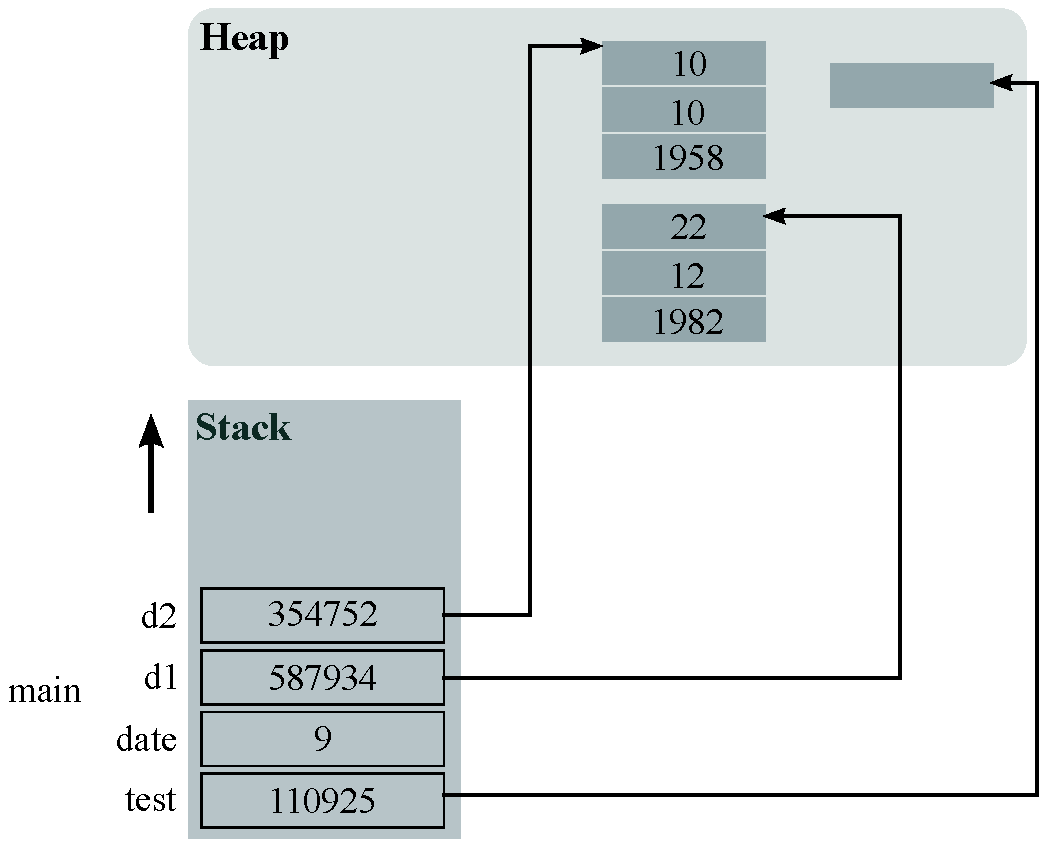
\includegraphics[width=0.98\textwidth]{fig01.pdf}
\end{figure}

\column{0.6\textwidth}  
\begin{javaCode}\small
public class Test {
  public static void main(String[] args) {
    Test test = new Test(); //1
    int data = 9; //2
    BirthDate d1 = new BirthDate(22, 12, 1982); //3
    BirthDate d2 = new BirthDate(10, 10, 1958); //4
    test.m1(data);
    test.m2(d1);
    test.m3(d2);
  }

  public void m1(int i) {
    i = 1234;
  }
  public void m2(BirthDate b) {
    b = new BirthDate(15, 6, 2010);
  }
  public void m3(BirthDate b) {
    b.setDay(18);
  }
}
\end{javaCode}
\end{columns}
\end{frame}



\begin{frame}[fragile] % [fragile]参数使得能够插入代码
\frametitle{程序调用过程(二)}

\begin{columns}
\column{0.4\textwidth} 
\begin{figure}
\centering
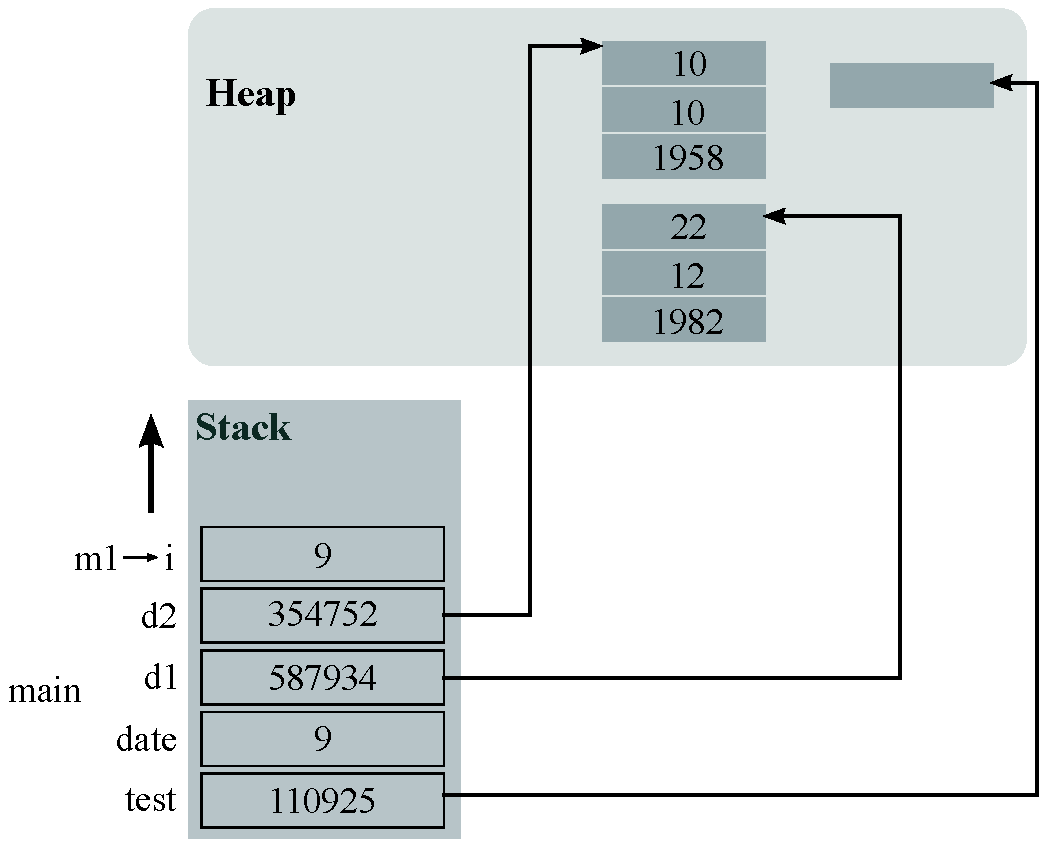
\includegraphics[width=0.98\textwidth]{fig02.pdf}
\end{figure}

\column{0.6\textwidth}  
\begin{javaCode}\small
public class Test {
  public static void main(String[] args) {
    Test test = new Test(); 
    int data = 9; 
    BirthDate d1 = new BirthDate(22, 12, 1982); 
    BirthDate d2 = new BirthDate(10, 10, 1958); 
    test.m1(data); //5
    test.m2(d1);
    test.m3(d2);
  }

  public void m1(int i) {
    i = 1234;
  }
  public void m2(BirthDate b) {
    b = new BirthDate(15, 6, 2010);
  }
  public void m3(BirthDate b) {
    b.setDay(18);
  }
}
\end{javaCode}
\end{columns}
\end{frame}



\begin{frame}[fragile] % [fragile]参数使得能够插入代码
\frametitle{程序调用过程(三)}

\begin{columns}
\column{0.4\textwidth} 
\begin{figure}
\centering
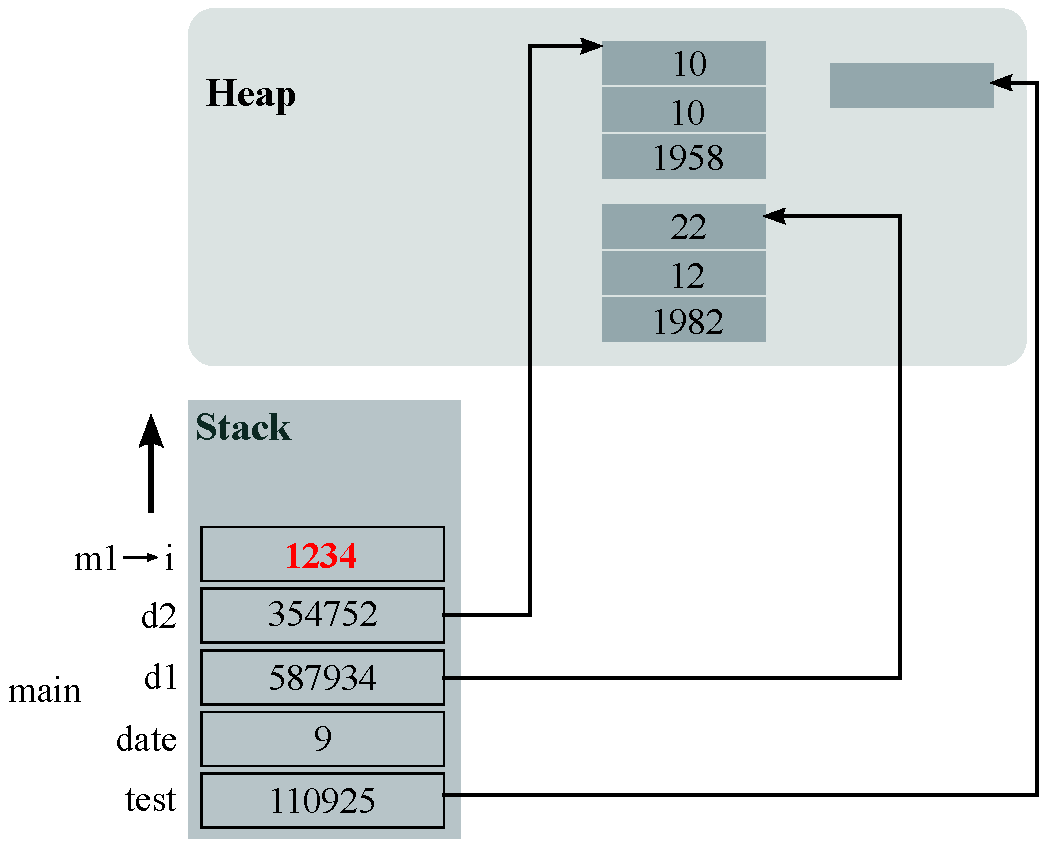
\includegraphics[width=0.98\textwidth]{fig03.pdf}
\end{figure}

\column{0.6\textwidth}  
\begin{javaCode}\small
public class Test {
  public static void main(String[] args) {
    Test test = new Test(); 
    int data = 9; 
    BirthDate d1 = new BirthDate(22, 12, 1982); 
    BirthDate d2 = new BirthDate(10, 10, 1958); 
    test.m1(data); 
    test.m2(d1);
    test.m3(d2);
  }

  public void m1(int i) {
    i = 1234; //6
  }
  public void m2(BirthDate b) {
    b = new BirthDate(15, 6, 2010);
  }
  public void m3(BirthDate b) {
    b.setDay(18);
  }
}
\end{javaCode}
\end{columns}
\end{frame}



\begin{frame}[fragile] % [fragile]参数使得能够插入代码
\frametitle{程序调用过程(四)}

\begin{columns}
\column{0.4\textwidth} 
\begin{figure}
\centering
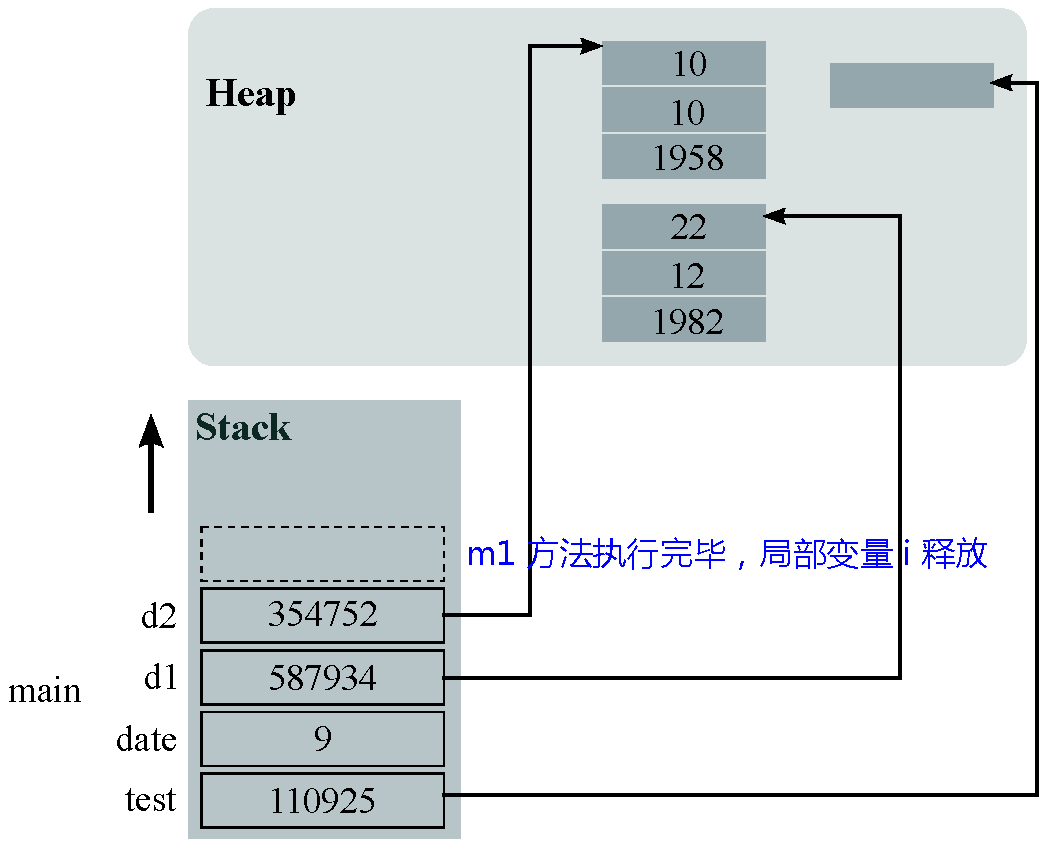
\includegraphics[width=0.98\textwidth]{fig04.pdf}
\end{figure}

\column{0.6\textwidth}  
\begin{javaCode}\small
public class Test {
  public static void main(String[] args) {
    Test test = new Test(); 
    int data = 9; 
    BirthDate d1 = new BirthDate(22, 12, 1982); 
    BirthDate d2 = new BirthDate(10, 10, 1958); 
    test.m1(date); 
    test.m2(d1); 
    test.m3(d2);
  }

  public void m1(int i) {
    i = 1234; 
  }
  public void m2(BirthDate b) {
    b = new BirthDate(15, 6, 2010);
  }
  public void m3(BirthDate b) {
    b.setDay(18);
  }
}
\end{javaCode}
\end{columns}
\end{frame}



\begin{frame}[fragile] % [fragile]参数使得能够插入代码
\frametitle{程序调用过程(五)}

\begin{columns}
\column{0.4\textwidth} 
\begin{figure}
\centering
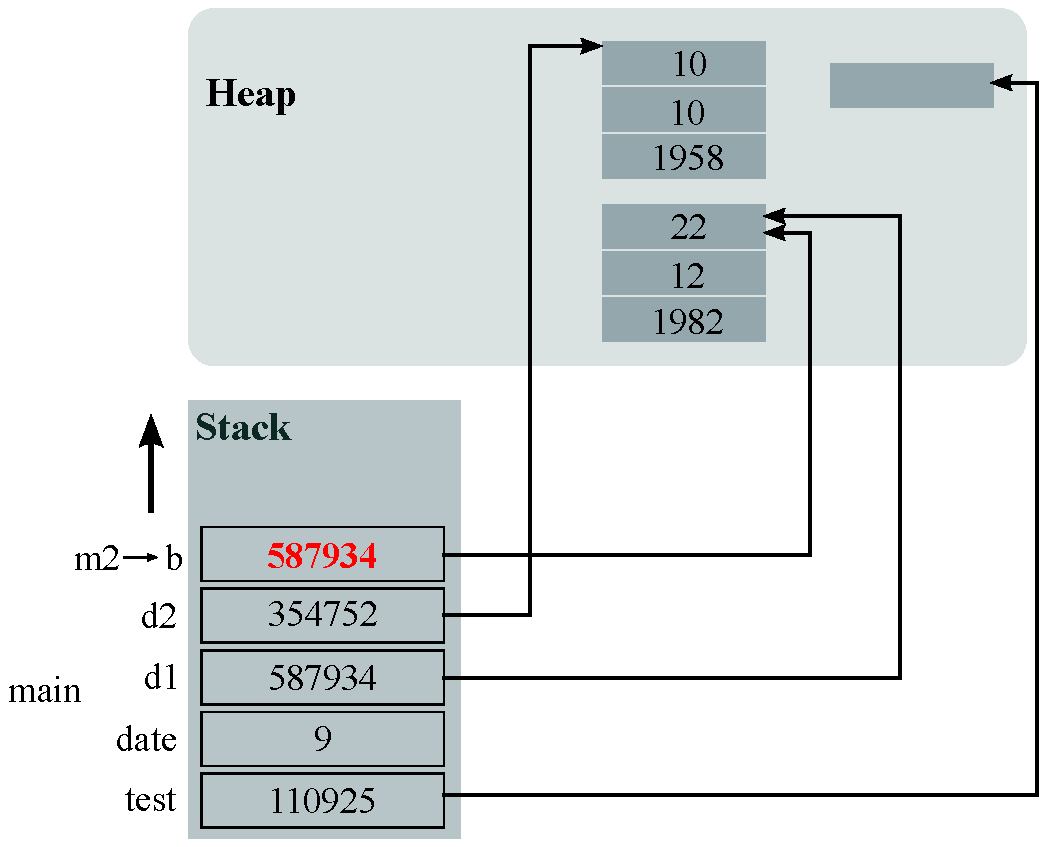
\includegraphics[width=0.98\textwidth]{fig05.pdf}
\end{figure}

\column{0.6\textwidth}  
\begin{javaCode}\small
public class Test {
  public static void main(String[] args) {
    Test test = new Test(); 
    int data = 9; 
    BirthDate d1 = new BirthDate(22, 12, 1982); 
    BirthDate d2 = new BirthDate(10, 10, 1958); 
    test.m1(data); 
    test.m2(d1); //7
    test.m3(d2);
  }

  public void m1(int i) {
    i = 1234; 
  }
  public void m2(BirthDate b) { 
    b = new BirthDate(15, 6, 2010);
  }
  public void m3(BirthDate b) {
    b.setDay(18);
  }
}
\end{javaCode}
\end{columns}
\end{frame}



\begin{frame}[fragile] % [fragile]参数使得能够插入代码
\frametitle{程序调用过程(六)}

\begin{columns}
\column{0.4\textwidth} 
\begin{figure}
\centering
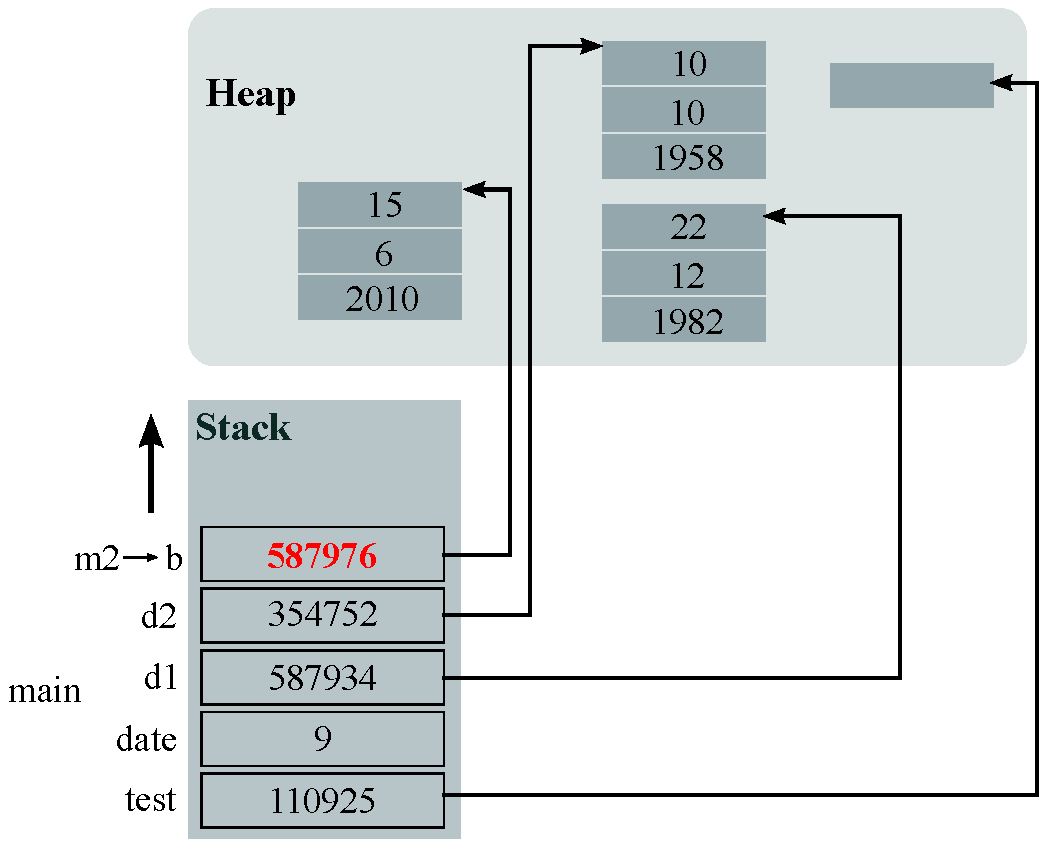
\includegraphics[width=0.98\textwidth]{fig06.pdf}
\end{figure}

\column{0.6\textwidth}  
\begin{javaCode}\small
public class Test {
  public static void main(String[] args) {
    Test test = new Test(); 
    int data = 9; 
    BirthDate d1 = new BirthDate(22, 12, 1982); 
    BirthDate d2 = new BirthDate(10, 10, 1958); 
    test.m1(data); 
    test.m2(d1); 
    test.m3(d2);
  }

  public void m1(int i) {
    i = 1234; 
  }
  public void m2(BirthDate b) { 
    b = new BirthDate(15, 6, 2010); //8
  }
  public void m3(BirthDate b) {
    b.setDay(18);
  }
}
\end{javaCode}
\end{columns}
\end{frame}

%%%\begin{frame}[fragile] % [fragile]参数使得能够插入代码
%%%\frametitle{程序调用过程(一)}
%%%\begin{itemize}
%%%\item JVM自动寻找main方法,执行第一句代码,创建一个Test类的实例,在栈中分配一块内存,存放
%%%  一个指向堆区对象的指针110925。
%%%\item 创建一个int型的变量data,由于是基本类型,直接在栈中存放data对应的值9。
%%%\item 创建两个BirthDate类的实例d1、d2,在栈中分别存放了对应的指针指向各自的对象。它们在实
%%%  例化时调用了有参数的构造方法,因此对象中有自定义初始值。
%%%\end{itemize}
%%%\end{frame}
%%%
%%%\begin{frame}[fragile] % [fragile]参数使得能够插入代码
%%%\frametitle{程序调用过程(二)}
%%%\begin{itemize}
%%%\item 调用test对象的m1方法,以data为参数。JVM读取这段代码时,检测到i是局部变量,则会把i放
%%%  在栈中,并且把data的值赋给i。
%%%\end{itemize}
%%%\end{frame}
%%%
%%%\begin{frame}[fragile] % [fragile]参数使得能够插入代码
%%%\frametitle{程序调用过程(三)}
%%%\begin{itemize}
%%%\item 把1234赋值给i。
%%%\end{itemize}
%%%\end{frame}
%%%
%%%\begin{frame}[fragile] % [fragile]参数使得能够插入代码
%%%\frametitle{程序调用过程(四)}
%%%\begin{itemize}
%%%\item m1方法执行完毕,立即释放局部变量i所占用的栈空间。。
%%%\end{itemize}
%%%\end{frame}
%%%
%%%\begin{frame}[fragile] % [fragile]参数使得能够插入代码
%%%\frametitle{程序调用过程(五)}
%%%\begin{itemize}
%%%\item 调用test对象的m2方法,以实例d1为参数。JVM检测到m2方法中的b参数为局部变量,立即加入
%%%  到栈中,由于是引用类型的变量,所以b中保存的是d1中的指针,此时b和d1指向同一个堆中的对象。
%%%  在b和d1之间传递是指针。
%%%\end{itemize}
%%%\end{frame}
%%%
%%%\begin{frame}[fragile] % [fragile]参数使得能够插入代码
%%%\frametitle{程序调用过程(六)}
%%%\begin{itemize}
%%%\item m2方法中又实例化了一个BirthDate对象,并且赋给b。在内部执行过程是:在堆区new了一个对
%%%  象,并且把该对象的指针保存在栈中b对应空间,此时实例b不再指向实例d1所指向的对象,但是实
%%%  例d1所指向的对象并无变化,未对d1造成任何影响。
%%%\end{itemize}
%%%\end{frame}
%%%
%%%\begin{frame}[fragile] % [fragile]参数使得能够插入代码
%%%\frametitle{程序调用过程(七)}
%%%\begin{itemize}
%%%\item m2方法执行完毕,立即释放局部引用变量b所占的栈空间,注意只是释放了栈空间,堆空间要等待自动回收。
%%%\end{itemize}
%%%\end{frame}
%%%
%%%\begin{frame}[fragile] % [fragile]参数使得能够插入代码
%%%\frametitle{程序调用过程(八)}
%%%\begin{itemize}
%%%\item 调用test实例的m3方法,以实例d2为参数。JVM会在栈中为局部引用变量b分配空间,并且
%%%  把d2中的指针存放在b中,此时d2和b指向同一个对象。再调用实例b的setDay方法,其实就是调
%%%  用d2指向的对象的setDay方法。
%%%\item 调用实例b的setDay方法会影响d2,因为二者指向的是同一个对象。
%%%\item m3方法执行完毕,立即释放局部引用变量b。
%%%\end{itemize}
%%%\end{frame}

\begin{frame}[fragile] % [fragile]参数使得能够插入代码

  \frametitle{Java程序运行内存分析小结}
  \begin{itemize}[<+-| structure@+>]\kai
  \item 基本类型和引用类型,二者作为局部变量时都存放在栈中。
  \item 基本类型直接在栈中保存值,引用类型在栈中保存一个指向堆区的指针,
    真正的对象存放在堆中。
  \item 作为参数时基本类型就直接传值,引用类型传指针。
  \end{itemize}

  \pause
  
  \notice{注意什么是对象}
  
  \begin{javaCode}
    MyClass a = new MyClass();
  \end{javaCode}
  
  此时a是指向对象的指针,而不能说a是对象。指针存储在栈中,对象存储在堆
  中,操作实例实际上是通过指针间接操作对象。多个指针可以指向同一个对
  象。

\end{frame}

\begin{frame}[fragile] % [fragile]参数使得能够插入代码
  \frametitle{Java程序运行内存分析小结}

  \begin{itemize}[<+-| structure@+>]\kai
  \item {\hei\Red 栈中的数据和堆中的数据销毁并不是同步的。}\only<1>{方法一旦执行结
      束,栈中的局部变量立即销毁,但是堆中对象不一定销毁。因为可能有其
      他变量也指向了这个对象,直到栈中没有变量指向堆中的对象时,它才销
      毁;而且还不是马上销毁,要等垃圾回收扫描时才可以被销毁。}
    
  \item {\hei\Red 栈、堆、代码段、数据段等都是相对于应用程序而言的。}\only<2>{每一
      个应用程序都对应唯一的一个JVM实例,每一个JVM实例都有自己的内存区
      域,互不影响,并且这些内存区域是该JVM实例所有线程共享的。}
  \end{itemize}
\end{frame}

\section{Java内存管理建议}

\begin{frame}[fragile] % [fragile]参数使得能够插入代码
\frametitle{Java垃圾回收机制} 

{\hei\Blue JVM的垃圾回收机制(GC)决定对象是否是垃圾对象,并进行回收。}

\wxd{垃圾回收机制的特点}

\begin{itemize}
\item 垃圾内存并不是用完了马上就被释放,所以会产生内存释放不及时的现象,
  从而降低内存的使用效率。而当程序庞大的时候,这种现象更为明显。
\item 垃圾回收工作本身需要消耗资源,同样会产生内存浪费。
\end{itemize}

%%%\wxd{JVM中的对象生命周期}\\
%%%对象的生命周期一般分为7个阶段:\ding{182}创建阶段、\ding{183}应用阶
%%%段、\ding{184}不可视阶段、\ding{185}不可到达阶段、\ding{186}可收集阶
%%%段、\ding{187}终结阶段、\ding{188}释放阶段。
\end{frame}

\begin{frame}[fragile] % [fragile]参数使得能够插入代码
\frametitle{Java人为的内存管理是必要的} 

\notice{Java需要内存管理}

\begin{itemize}
\item 虽然JVM已经代替开发者完成了对内存的管理,但是硬件本身的资源是有限的。
\item 如果Java的开发人员不注意内存的使用依然会造成较高的内存消耗,导致性能的降低。
\end{itemize}

\end{frame}


\begin{frame}[fragile] % [fragile]参数使得能够插入代码
\frametitle{JVM内存溢出和参数调优}

\notice{当遇到OutOfMemoryError时该如何做?}

\begin{itemize}[<+-| structure@+>]
\item 常见的OOM(Out Of Memory)内存溢出异常,就是堆内存空间不足以存放新对象实例时导致。
\item 永久区内存溢出相对少见,一般是由于需要加载海量的Class数据,超过了
  非堆内存的容量导致。
  %通常出现在Web应用刚刚启动时。因此Web应用推荐使用
  %预加载机制,方便在部署时就发现并解决该问题。
 \item 栈内存也会溢出,但是更加少见。
\end{itemize}

\xyy{处理方法} \ding{182} 调整JVM内存配置;\ding{183} 优化代码


\pause
\begin{description}\scriptsize
\item[堆内存优化] 调整JVM启动参数-Xms -Xmx -XX:newSize -XX:MaxNewSize,如调整初始堆内存和
  最大对内存 -Xms256M -Xmx512M。 或者调整初始New Generation的初始内存和最大内
  存 -XX:newSize=128M -XX:MaxNewSize=128M。
 \item[永久区内存优化] 调整PermSize参数   如  -XX:PermSize=256M -XX:MaxPermSize=512M。
 \item[栈内存优化] 调整每个线程的栈内存容量  如  -Xss2048K。
\end{description}
\end{frame}

\begin{frame}[fragile] % [fragile]参数使得能够插入代码
  \frametitle{内存优化的小示例}

  \wxd{减少无谓的对象引用创建}

  \samp{Test 1}

  \begin{javaCode}
    for(int i=0; i<10000; i++) {
      Object obj = new Object(); 
    }
  \end{javaCode}
  
  \samp{Test 2}
  
  \begin{javaCode}
    Object obj = null; 
    for( int i=0; i<10000; i++) {
      obj = new Object(); 
    }
  \end{javaCode}

  \pause 
  \xyy{内存性能分析}
  
  {\small\kai Test 2比Test 1的性能要好。两段程序每次执行for循环都要创建
    一个Object的临时对象,JVM的垃圾回收不会马上销毁但这些临时对象。相对
    于Test 1,Test 2则只在栈内存中保存一份对象的引用,而不必创建大量新临
    时变量,从而降低了内存的使用。}
\end{frame}

\begin{frame}[fragile] % [fragile]参数使得能够插入代码
  \frametitle{内存优化的小示例}
  \wxd{不要对同一对象初始化多次}

  \begin{javaCode}
    public class A { 
      private Hashtable table = new Hashtable(); 
      public A() { 
        table = new Hashtable();
      }
    }
  \end{javaCode}

  \pause
  \xyy{内存性能分析}

  {\small\kai 上述代码new了两个Hashtable,但是却只使用了一个,另外一个
    则没有被引用而被忽略掉,浪费了内存。并且由于进行了两次new操作,也影
    响了代码的执行速度。另外,不要提前创建对象,尽量在需要的时候创建对
    象。}
\end{frame}

%%%\begin{frame}[fragile] % [fragile]参数使得能够插入代码
%%%\frametitle{其他阶段}
%%%\begin{description}
%%%\item[应用] 即该对象至少有一个引用在维护它。
%%%\item[不可视] 即超出该变量的作用域。\\{\kai 因为JVM GC并不是马上进行回收,而是要判断对象
%%%    是否被其他引用维护。所以,如果我们在使用完一个对象以后对其进行obj =
%%%    null或者obj.doSomething()操作,将其标记为空,则帮助JVM及时发现这个垃圾对象。}
%%%\item[不可到达] 即在JVM中找不到对该对象的直接或者间接的引用。
%%%\item[可收集,终结,释放] 垃圾回收器发现该对象不可到达,finalize方法已经被执
%%%  行,或者对象空间已被重用的时候。
%%%\end{description}
%%%\end{frame}


%%%\begin{frame}[fragile] % [fragile]参数使得能够插入代码
%%%  \frametitle{Java的finalize()方法}
%%%
%%%Java所有类都继承自Object类,而finalize()是Object类的一个函数,该函数在Java中类似于C++的析
%%%构函数(仅仅是类似)。一般来说可以通过重载finalize()的形式来释放类中对象。
%%%
%%%\begin{javaCode}
%%%public class A { 
%%%  public Object a; 
%%%
%%%  public A() { 
%%%    a = new Object() ;
%%%  } 
%%%  
%%%  protected void finalize() throws java.lang.Throwable { 
%%%    a = null; // 标记为空,释放对象 
%%%    super.finalize(); // 递归调用超类中的 finalize 方法
%%%  }
%%%} 
%%%\end{javaCode}
%%%
%%%什么时候finalize()被调用由JVM来决定。{\hei\Blue 尽量少用finalize()函
%%%  数,finalize()函数是Java提供给程序员一个释放对象或资源的机会。但它会
%%%  加大GC的工作量,因此尽量少采用finalize方式回收资源。}
%%%\end{frame}

%%%\begin{frame}[fragile] % [fragile]参数使得能够插入代码
%%%  \frametitle{Java的finalize()方法}
%%%  \begin{itemize}
%%%  \item 一般的,纯Java编写的Class不需要重写finalize()方法,因为Object已
%%%    经实现了一个默认的,除非我们要实现特殊的功能。
%%%  \item 用Java以外的代码编写的Class(比如JNI、C++的new方法分配的内存),
%%%    垃圾回收器并不能对这些部分进行正确的回收,这就需要我们覆盖默认的方
%%%    法来实现对这部分内存的正确释放和回收。
%%%  \end{itemize}
%%%\end{frame}

%%%\section{常量池}
%%%
%%%\begin{frame}[fragile]
%%%  \frametitle{常量池}
%%%
%%%  \notice{常量池部分为课后选择性自学部分,对常量池的基本理解有助于加深对Java内存模型的认识。}
%%%  
%%%  \wxd{常量池分类}
%%%
%%%  \begin{itemize}
%%%  \item 全局字符串常量池(string literal pool)
%%%  \item class文件常量池(class constant pool)
%%%  \item 运行时常量池(runtime constant pool)
%%%  \end{itemize}
%%%\end{frame}
%%%
%%%\begin{frame}[fragile] % [fragile]参数使得能够插入代码
%%%\frametitle{基本类型和基本类型的包装类}
%%%
%%%\wxd{基本类型}\\
%%%byte、short、char、int、long、boolean
%%%
%%%\wxd{基本类型的包装类}\\
%%%Byte、Short、Character、Integer、Long、Boolean
%%%
%%%\wxd{二者的区别}\\
%%%基本类型体现在程序中是普通变量,基本类型的包装类是类,体现在程序中是引用变量。因此二者在内存中的存储位置不同:基本类型存储在栈中,而基本类型包装类存储在堆中。
%%%
%%%{\hei 上述包装类均实现了常量池技术,另外两种浮点数类型的包装类则没有实现。String类型也实现了常量池技术。}
%%%\end{frame}
%%%
%%%\begin{frame}[fragile] % [fragile]参数使得能够插入代码
%%%\frametitle{代码实例}
%%%\begin{javaCode}
%%%public class Test {
%%%  public static void main(String[] args) {    
%%%    objPoolTest();
%%%  }
%%%  
%%%  public static void objPoolTest() {
%%%    int i = 40;
%%%    int i0 = 40;
%%%    Integer i1 = 40;
%%%    Integer i2 = 40;
%%%    Integer i3 = 0;
%%%    Integer i4 = new Integer(40);
%%%    Integer i5 = new Integer(40);
%%%    Integer i6 = new Integer(0);
%%%    Double d1 = 1.0;
%%%    Double d2 = 1.0;
%%%        
%%%    System.out.println("i=i0\t" + (i == i0));
%%%    System.out.println("i1=i2\t" + (i1 == i2));
%%%    System.out.println("i1=i2+i3\t" + (i1 == i2 + i3));
%%%    System.out.println("i4=i5\t" + (i4 == i5));
%%%    System.out.println("i4=i5+i6\t" + (i4 == i5 + i6));    
%%%    System.out.println("d1=d2\t" + (d1==d2)); 
%%%    System.out.println();        
%%%  }
%%%}  
%%%\end{javaCode}
%%%\end{frame}
%%%
%%%\begin{frame}[fragile] % [fragile]参数使得能够插入代码
%%%\frametitle{Output}
%%%\begin{stdoutCode}
%%%i=i0    true
%%%i1=i2   true
%%%i1=i2+i3    true
%%%i4=i5   false
%%%i4=i5+i6    true
%%%d1=d2   false  
%%%\end{stdoutCode}
%%%\end{frame}
%%%
%%%\begin{frame}[fragile] % [fragile]参数使得能够插入代码
%%%\frametitle{Output分析}
%%%
%%%\begin{itemize}[<+-| structure@+>]\kai
%%%\item i和i0均是普通类型(int)的变量,所以数据直接存储在栈中,而栈有一个很重要的特性:{\Blue 栈
%%%  中的数据可以共享}。当我们定义了int i = 40;,再定义int i0 = 40;,这时候会自动检查栈中是否
%%%  有40这个数据,如果有,i0会直接指向i的40,不会再添加一个新的40。
%%%\item i1和i2均是引用类型,在栈中存储指针,因为Integer是包装类,实现了常量池技术,因
%%%  此i1、i2的40均是从常量池中获取的,均指向同一个地址,因此i1 = i2。
%%%\item 很明显这是一个加法运算,Java的数学运算都是在栈中进行的,Java会自动对i1、i2进行拆箱
%%%  操作转化成整型,因此i1在数值上等于i2 + i3。
%%%\end{itemize}
%%%\end{frame}
%%%
%%%\begin{frame}[fragile] % [fragile]参数使得能够插入代码
%%%\frametitle{Output分析}
%%%\begin{itemize}[<+-| structure@+>]\kai
%%%\item i4和i5均是引用类型,在栈中存储指针,因为Integer是包装类。但是由于他们各自都是new出
%%%  来的,因此不再从常量池寻找数据,而是从堆中各自new一个对象,然后各自保存指向对象的指针,
%%%  所以i4和i5不相等,因为他们所存指针不同,所指向对象不同。
%%%\item 也是一个加法运算,同理3。
%%%\item d1和d2均是引用类型,在栈中存储指针,因为Double是包装类。但{\Red Double包装类没有实现常量
%%%  池技术},因此Double d1 = 1.0;相当于Double d1 = new Double(1.0);,是在堆中new一个对象,d2同理。
%%%  因此d1和d2存放的指针值不同,指向的对象不同,所以不相等。
%%%\end{itemize}
%%%\end{frame}
%%%
%%%\begin{frame}[fragile] % [fragile]参数使得能够插入代码
%%%\frametitle{Output分析}
%%%\begin{itemize}[<+-| structure@+>]\kai
%%%\item 以上提到的几种基本类型包装类均实现了常量池技术,但他们{\Red 维护的常量仅仅是
%%%    从-128至127这个范围内},如果常量值超过这个范围,就会从堆中创建对象,不再从常量池中取。
%%%  比如,把上边例子改成Integer i1 = 400; Integer i2 = 400;,很明显超过了127,无法从常量池
%%%  中获取常量,就要从堆中new新的Integer对象,这时i1和i2就不相等。
%%%\item String类型也实现了常量池技术,但是稍有不同。String型是先检测常量池中有没有对应字符
%%%  串,如果有则取出来;如果没有则把当前的添加进去。
%%%\begin{javaCode}
%%%// s1, s2 分别位于堆中不同空间
%%%String s1 = new String("hello");
%%%String s2 = new String("hello");
%%%System.out.println(s1 == s2); // 输出 false
%%%// s3, s4 位于池中同一空间
%%%String s3 = "hello";
%%%String s4 ="hello";
%%%System.out.println(s3 == s4);// 输出 true
%%%\end{javaCode}
%%%\end{itemize}
%%%\end{frame}


%%%%%%%%%%%%%%%%%%%%%%%%%%%%%%%%%%%%%%%%%%%%%%%%%%%
\begin{frame}
  \frametitle{本节习题}

  \wxd{简答题}
  \begin{enumerate}
  \item 请描述JVM的内存模型。
  \item 搜索关于Java中比较操作“==”和“equals()”的相关文档,并进行总结,加
    深对Java内存模型的理解。
  \item 搜索关于Java常量池技术的相关文档和资源,并进行总结。(选做)
  \end{enumerate}

  \wxd{小编程}
  \begin{enumerate}
  \item 编写Java程序内存运行分析部分的程序,通过调试模式跟踪查看内存的变化情况。
  \end{enumerate}
\end{frame}
%%%%%%%%%%%%%%%%%%%%%%%%%%%%%%%%%%%%%%%%%%%%%%%%%%%%%%%%%%%%%%%%%%%%%%%%%%%%%%%
% TKS Page %%%%%%%%%%%%%%%%%%%%%%%%%%%%%%%%%%%%%%%%%%%%
\begin{frame}
\centering
{\Huge \textcolor{blue}{THE END}} \\
\vspace{5mm}
{\Large wangxiaodong@ouc.edu.cn} \\
\end{frame}
%%%%%%%%%%%%%%%%%%%%%%%%%%%%%%%%%%%%%%%%%%%%%%%%%%%%%%%
%%%%%%%%%%%%%%%%%%%%%%%%%%%%%%%%%%%%%%%%%%%%%%%%%%%%%%%%%%%%%%%%%%%%%%%%%%%%%%%
\end{document}